\chapter*{Introduction}
\phantomsection
\addstarredchapter{\textbf{Introduction}}

\fancyhead[LE]{\thepage}
\fancyhead[RE]{\textbf{Introduction}}
\fancyhead[RO]{\thepage}
\fancyhead[LO]{\textbf{Introduction}}
\fancyfoot[C]{\thepage}

\setlength{\parindent}{0.35cm}

% ====================================================

L'outil de visualisation \cwv~a été développé dans le but de visualiser les sorties de modélisation de la plate-forme de modélisation \cws\cwversion. Cette extension fonctionne actuellement comme un plug-in QGIS sous la version \qgisversion de QGIS, et les mêmes fonctionnalités sont également accessibles par API à travers un notebook Jupyter \label{sec-notebook-usage}.\\

\cwv~s'articule autour de différents outils et fonctionnalités qui accompagnent le processus de calage d'une application \cawaqs~et facilitent la visualisation des chroniques temporelles et de la distribution spatiale des variables hydrologiques simulées.

\cwv~s'appuie sur un backend scientifique autonome, HTAS \href{https://github.com/flipoyo/HydrologicalTwinAlphaSeries}{(HydrologicalTwinAlphaSeries)}, qu'il consomme au travers d'une interface publique bien définie.

La \cref{fig-cvz-ecosystem} situe le plug-in au sein de la chaîne d'outils \cawaqs.
\begin{figure}[H]
    \centering
    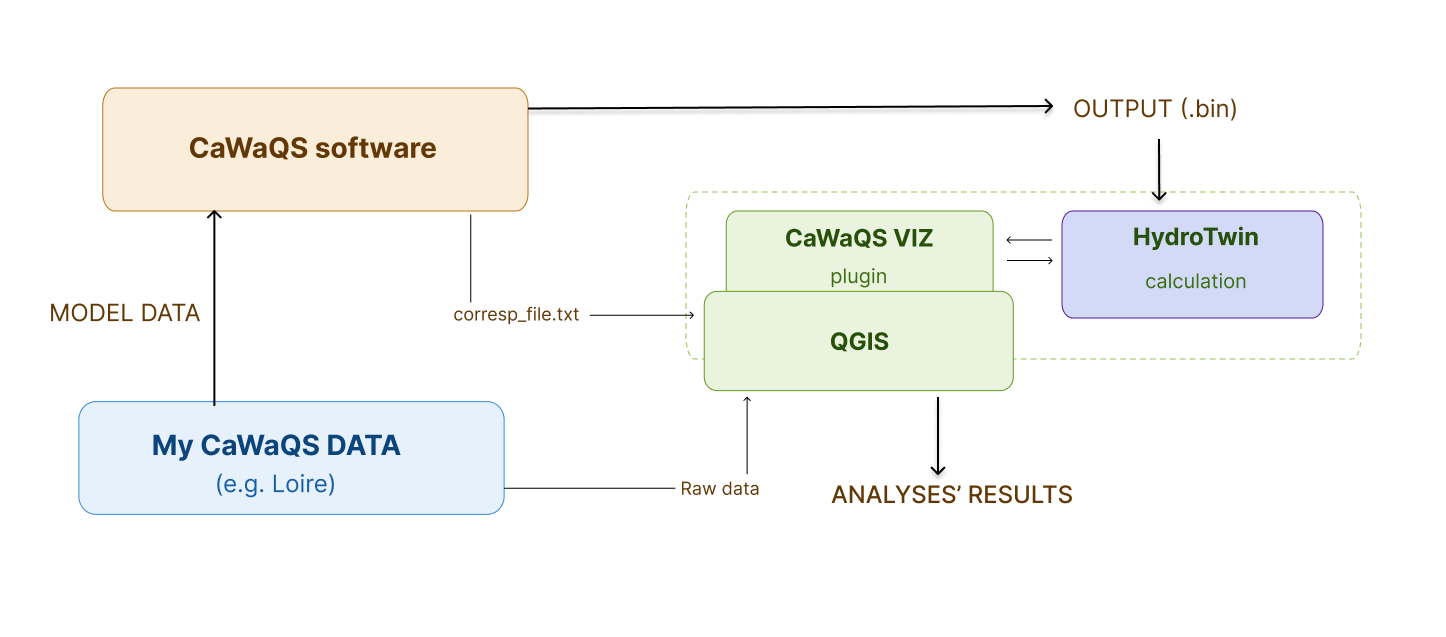
\includegraphics[width=0.9\linewidth]{0_introduction/fig/cvz_ecosystem.png}
    \caption{L'écosystème \cwv~--- position du plug-in au sein de la chaîne d'outils \cawaqs.}
    \label{fig-cvz-ecosystem}
\end{figure}
